\documentclass[11pt]{article}

\usepackage[paperwidth=28cm, paperheight=21cm, margin=2.5cm]{geometry}
\usepackage{fontspec}
\usepackage[spanish, bidi=basic, provide=*]{babel}
\babelprovide[import, onchar=ids fonts]{english}
\babelfont{rm}{Noto Sans}
\usepackage{enumitem}
\setlist[itemize]{label=-}
\usepackage{amsmath, amssymb}
\usepackage{booktabs}
\usepackage{graphicx}
\usepackage{xcolor}
\usepackage{hyperref}

\definecolor{accentblue}{RGB}{24, 78, 119}
\definecolor{mutedgray}{RGB}{85, 95, 105}

\hypersetup{
    colorlinks=true,
    linkcolor=accentblue,
    urlcolor=accentblue,
    pdftitle={Explicacion fisica y numerica de perfil_radial_baja_frecuencia_v2.py},
}

\title{\textbf{\color{accentblue}Explicación física y numérica del script \texttt{perfil\_radial\_baja\_frecuencia\_v2.py}}}
\author{Documentación técnica --- Electromagnetismo}
\date{}

\begin{document}

\maketitle

\begin{abstract}
Este documento detalla los fundamentos electromagnéticos y los algoritmos numéricos empleados en el script \texttt{perfil\_\allowbreak radial\_\allowbreak baja\_\allowbreak frecuencia\_\allowbreak v2.py} para calcular y representar el perfil radial exacto del campo magnético cuasiestático $H_\phi(\rho, z)$ en un condensador de placas circulares paralelas. Se describen la reducción de Biot-Savart mediante el teorema de Helmholtz, la evaluación cerrada de la integral acimutal con integrales elípticas completas y la resolución numérica de la ecuación integral de Love (1949) para placas conductoras equipotenciales, incluyendo el cambio de variable que elimina la singularidad de borde.
\end{abstract}

\tableofcontents
\vspace{0.4cm}

\section{Objetivo, geometría y normalización}

El script calcula el campo magnético acimutal $H_\phi(\rho, z) = B_\phi(\rho, z)/\mu_0$ en régimen de baja frecuencia o cuasiestático ($kR = \omega R / c \ll 1$) para un condensador formado por dos discos paralelos de radio $R$ situados en $z = +d/2$ y $z = -d/2$, alimentados por dos conductores rectilíneos sobre el eje $z$ por los que desciende una corriente $I(t)$ en sentido $-\hat{z}$.

Todas las longitudes se adimensionalizan tomando $R = 1$ y definiendo la relación de aspecto $\kappa = d/R$ (por defecto \texttt{D\_OVER\_R = 0.2}). El campo magnético se normaliza respecto al valor de referencia en el borde de la placa:
\begin{equation}
    H_0 = \frac{I}{2\pi R}.
\end{equation}
Con esta normalización:
\begin{itemize}
    \item El campo de un hilo rectilíneo infinito, $H_{\mathrm{inf}}(\rho) = I / (2\pi\rho)$, se reduce a $H_{\mathrm{inf}}/H_0 = R/\rho$ y vale exactamente $1$ en $\rho = R$.
    \item El límite ideal sin efectos de borde ($d \ll R$) viene dado por $\rho/R$ en el interior ($\rho \le R$) y por $R/\rho$ en el exterior ($\rho > R$).
    \item Los dos planos evaluados son el plano medio entre placas (\texttt{Z\_MID = 0.0}) y un plano situado a $5d$ por encima de la placa superior (\texttt{Z\_TOP\_5D = 0.5*d + 5.0*d = 5.5*d}).
\end{itemize}

\section{Reducción a corrientes de conducción (teorema de Helmholtz)}

En régimen cuasiestático, la inducción de Faraday es despreciable ($\nabla \times \mathbf{E} \approx \mathbf{0}$), por lo que el campo eléctrico deriva de un potencial escalar $\mathbf{E} = -\nabla\phi$. En consecuencia, la densidad de corriente de desplazamiento $\mathbf{J}_d = \varepsilon_0 \partial_t \mathbf{E}$ es estrictamente irrotacional:
\begin{equation}
    \nabla \times \mathbf{J}_d = -\varepsilon_0 \nabla \times \nabla\left(\frac{\partial \phi}{\partial t}\right) = \mathbf{0}.
\end{equation}
Por el teorema de Helmholtz, la integral de Biot-Savart de un campo vectorial irrotacional que decae suficientemente rápido en el infinito se anula idénticamente:
\begin{equation}
    \frac{1}{4\pi} \iiint \frac{\mathbf{J}_d(\mathbf{r}') \times (\mathbf{r} - \mathbf{r}')}{|\mathbf{r} - \mathbf{r}'|^3}\,dV' = \frac{1}{4\pi} \iiint \frac{\nabla' \times \mathbf{J}_d(\mathbf{r}')}{|\mathbf{r} - \mathbf{r}'|}\,dV' = \mathbf{0}.
\end{equation}
Por esta razón, el script no necesita calcular el campo eléctrico en todo el espacio ni integrar $\mathbf{J}_d$ en 3D: el campo magnético total exacto se obtiene sumando únicamente las contribuciones de Biot-Savart de las corrientes de conducción en los dos hilos semiinfinitos y en las dos placas circulares.

\section{Contribución de los hilos semiinfinitos (\texttt{H\_wire\_norm})}

Los dos conductores rectilíneos ocupan los intervalos $z' \in (-\infty, -d/2]$ y $z' \in [+d/2, +\infty)$ sobre el eje $z$. Integrando la ley de Biot-Savart a lo largo de ambos tramos y dividiendo por $H_0 = I/(2\pi R)$, se obtiene la expresión analítica implementada en \texttt{H\_wire\_norm(rho, z)}:
\begin{equation}
    \frac{H_{\mathrm{hilos}}(\rho, z)}{H_0} = \frac{R}{2\rho} \left( 2 + \frac{z - d/2}{\sqrt{\rho^2 + (z - d/2)^2}} - \frac{z + d/2}{\sqrt{\rho^2 + (z + d/2)^2}} \right).
\end{equation}
En el código se impone un umbral de seguridad (\texttt{rho < 1e-12}) que devuelve directamente $0$, evitando la división por cero sobre el eje de simetría.

\section{Contribución de las placas e integrales elípticas}

Sea $F(\rho') = I_{\mathrm{rad}}(\rho') / I$ la fracción de corriente total que fluye radialmente hacia fuera en la placa superior más allá de un radio $\rho' \in [0, R]$. Por conservación de la carga y simetría axial, la densidad de corriente superficial en cada placa ($z_p = \pm d/2$, con signo $s = \pm 1$) es:
\begin{equation}
    \mathbf{K}_s(\rho') = s\,\frac{I}{2\pi \rho'}\,F(\rho')\,\hat{\rho}'.
\end{equation}

Al evaluar Biot-Savart en un punto de observación $(\rho, 0, z)$ con distancia vertical $\Delta z = z - z_p$, el producto vectorial $\hat{\rho}' \times (\mathbf{r} - \mathbf{r}')$ proyectado sobre la dirección del campo acimutal $-\hat{\phi}$ aporta un factor $\Delta z \cos\varphi$, mientras que el factor $\rho'$ del elemento de área $\rho'\,d\rho'\,d\varphi$ se cancela exactamente con el denominador de $\mathbf{K}_s(\rho')$. Normalizando respecto a $H_0$, resulta la fórmula implementada en \texttt{H\_total\_norm}:
\begin{equation}
    \frac{H_{\mathrm{placa}, s}(\rho, z)}{H_0} = \frac{s\,R\,\Delta z}{4\pi} \int_{0}^{R} F(\rho')\,\Phi(\rho, \rho', \Delta z)\,d\rho',
\end{equation}
donde $\Phi(\rho, \rho', \Delta z)$ es la integral acimutal:
\begin{equation}
    \Phi(\rho, \rho', \Delta z) = \int_{0}^{2\pi} \frac{\cos\varphi}{\left( \rho^2 + \rho'^2 + \Delta z^2 - 2\rho\rho'\cos\varphi \right)^{3/2}}\,d\varphi.
\end{equation}

\subsection{Evaluación cerrada mediante integrales elípticas (\texttt{phi\_elliptic\_integral})}

Para evitar una doble cuadratura numérica costosa, el script evalúa $\Phi$ de forma exacta mediante las integrales elípticas completas de primera y segunda especie, $K(m)$ y $E(m)$ (\texttt{scipy.special.ellipk} y \texttt{ellipe}):
\begin{equation}
    \Phi(\rho, \rho', \Delta z) = \frac{4}{\left((\rho + \rho')^2 + \Delta z^2\right)^{3/2}} \left[ \frac{2 - m}{m(1 - m)}\,E(m) - \frac{2}{m}\,K(m) \right],
\end{equation}
con el parámetro elíptico:
\begin{equation}
    m = \frac{4\rho\rho'}{(\rho + \rho')^2 + \Delta z^2} \in [0, 1).
\end{equation}

\subsection{Cuadratura radial adaptativa (\texttt{H\_total\_norm})}

La integral restante en $\rho' \in [0, R]$ se calcula con \texttt{scipy.integrate.quad} usando tolerancias \texttt{epsabs = 1e-8} y \texttt{epsrel = 1e-8}. Cuando el punto de observación cae dentro del radio de las placas ($\rho < R$) y $|\Delta z|$ es pequeño, el integrando presenta un pico muy estrecho alrededor de $\rho' = \rho$. Por ello el código pasa explícitamente \texttt{points=[rho]} a \texttt{quad}, forzando al algoritmo adaptativo a subdividir el intervalo justo en el pico y garantizando convergencia estable.

\section{Modelos de corriente radial: $\sigma$ uniforme frente a Love (1949)}

El script permite comparar dos modelos físicos para la función de reparto radial $F(\rho')$:

\subsection{Modelo 1: densidad de carga uniforme (\texttt{F\_uniform})}

Si se supone una densidad superficial uniforme $\sigma(t) = Q(t)/(\pi R^2)$, la carga contenida dentro de un círculo de radio $\rho$ es $Q(\rho) = Q\,(\rho/R)^2$, por lo que la fracción de corriente que continúa hacia el exterior de la placa es:
\begin{equation}
    F_{\mathrm{unif}}(\rho) = 1 - \frac{\rho^2}{R^2} \qquad (\rho \le R).
\end{equation}
Este modelo captura el efecto geométrico del espesor finito $d/R$ (suavizando el pico en $\rho = R$ desde $1{,}000\,H_0$ hasta $0{,}785\,H_0$ para $d = 0{,}2\,R$), pero desprecia la acumulación electrostática de carga cerca del borde conductor.

\subsection{Modelo 2: discos conductores equipotenciales (\texttt{solve\_love\_equation})}

En un condensador metálico real, cada placa es una superficie equipotencial ($\pm V/2$) y la densidad de carga diverge de forma integrable en el borde como $\sigma(\rho) \propto (R^2 - \rho^2)^{-1/2}$. Love (1949) demostró que este problema electrostático se reduce exactamente a una ecuación integral de Fredholm de segunda especie para una función auxiliar par $f(x)$ en $[-1, 1]$:
\begin{equation}
    f(x) - \frac{1}{\pi} \int_{-1}^{1} \frac{\kappa}{\kappa^2 + (x - t)^2}\,f(t)\,dt = 1, \qquad \kappa = \frac{d}{R}.
    \label{eq:love}
\end{equation}

El método numérico implementado en \texttt{solve\_love\_equation} consta de tres pasos:

\begin{enumerate}
    \item \textbf{Discretización de Nyström con Gauss-Legendre:} mediante \texttt{leggauss(80)} se generan $N = 80$ nodos $t_j$ y pesos $w_j$ en $[-1, 1]$. La ecuación \eqref{eq:love} se convierte en el sistema lineal denso de dimensión $80 \times 80$:
    \begin{equation}
        \left( \mathbf{I} - \mathbf{K} \right) \mathbf{f} = \mathbf{1}, \qquad K_{ij} = \frac{1}{\pi}\,\frac{\kappa}{\kappa^2 + (t_i - t_j)^2}\,w_j,
    \end{equation}
    resuelto con \texttt{np.linalg.solve}. A partir de $I_f = \int_{-1}^{1} f(t)\,dt \approx \sum_{j=1}^{N} w_j f_j$, se obtiene la capacidad exacta respecto al condensador ideal:
    \begin{equation}
        \frac{C}{C_{\mathrm{ideal}}} = \frac{2\kappa}{\pi}\,I_f.
    \end{equation}
    Para $\kappa = 0{,}2$, el script obtiene $C / C_{\mathrm{ideal}} = 1{,}3180$.

    \item \textbf{Interpolación exacta fuera de los nodos (\texttt{eval\_f}):} para evaluar $f(x)$ en cualquier $x \in [0, 1]$ sin pérdida de precisión, se emplea la propia ecuación integral (fórmula de Nyström):
    \begin{equation}
        f(x) = 1 + \frac{1}{\pi} \sum_{j=1}^{N} \frac{\kappa}{\kappa^2 + (x - t_j)^2}\,w_j f_j.
    \end{equation}

    \item \textbf{Eliminación de la singularidad en $F_{\mathrm{Love}}(\rho)$:} en el formalismo de Love, la fracción de corriente radial para $u = \rho/R \in [0, 1)$ viene dada por:
    \begin{equation}
        F_{\mathrm{Love}}(\rho) = \frac{1}{\frac{1}{2} I_f} \int_{u}^{1} \frac{x\,f(x)}{\sqrt{x^2 - u^2}}\,dx,
    \end{equation}
    que presenta una singularidad integrable en el extremo inferior $x = u$. El código la elimina analíticamente mediante el cambio de variable:
    \begin{equation}
        x(s) = \sqrt{u^2 + (1 - u^2)s^2}, \qquad s \in [0, 1],
    \end{equation}
    para el cual $x\,dx = (1 - u^2)s\,ds$ y $\sqrt{x^2 - u^2} = s\sqrt{1 - u^2}$. El factor $s$ se cancela exactamente y la integral pasa a ser completamente suave:
    \begin{equation}
        F_{\mathrm{Love}}(\rho) = \frac{\sqrt{1 - u^2}}{\frac{1}{2} I_f} \int_{0}^{1} f\!\left( \sqrt{u^2 + (1 - u^2)s^2} \right) ds,
    \end{equation}
    que se evalúa con una cuadratura fija de Gauss-Legendre de 40 puntos trasladada al intervalo $[0, 1]$.
\end{enumerate}

Físicamente, al concentrarse más carga en la periferia de las placas metálicas, la corriente radial $F_{\mathrm{Love}}(\rho)$ es mayor que $F_{\mathrm{unif}}(\rho)$, lo que produce un campo magnético interior aún más atenuado ($H_\phi(R, 0) \approx 0{,}744\,H_0$) y una pendiente inicial cercana a $C_{\mathrm{ideal}}/C \approx 0{,}759$.

\section{Estructura del código y generación de figuras (\texttt{main})}

La Tabla~\ref{tab:funciones} resume la arquitectura modular del script.

\begin{table}[ht]
\centering
\caption{Resumen de las funciones implementadas en \texttt{perfil\_radial\_baja\_frecuencia\_v2.py}.}
\label{tab:funciones}
\begin{tabular}{@{}p{4.3cm}p{10.9cm}@{}}
\toprule
\textbf{Función / bloque} & \textbf{Cometido físico y numérico} \\
\midrule
\texttt{solve\_love\_equation} & Resuelve la ecuación de Fredholm de Love (1949) por Nyström (80 nodos) y construye \texttt{F\_love(rho)} sin singularidad. \\
\texttt{F\_uniform} & Devuelve la distribución radial parabólica $1 - (\rho/R)^2$ asociada a carga uniforme. \\
\texttt{H\_wire\_norm} & Evalúa en forma cerrada el campo de los dos conductores semiinfinitos. \\
\texttt{phi\_elliptic\_integral} & Evalúa la integral acimutal de Biot-Savart mediante $K(m)$ y $E(m)$. \\
\texttt{H\_total\_norm} & Suma los hilos y la cuadratura adaptativa (\texttt{quad}) sobre ambas placas. \\
\texttt{main} & Construye la malla radial, calcula las cinco curvas y exporta la figura en PDF y PNG a 300 dpi. \\
\bottomrule
\end{tabular}
\end{table}

Respecto a la representación gráfica en \texttt{main}:
\begin{itemize}
    \item \textbf{Malla radial no uniforme:} se concatenan tres tramos en $\rho/R \in [0, 3]$ con mayor densidad en la región del borde $[0{,}85, 1{,}20]$ para describir con nitidez la curvatura del máximo.
    \item \textbf{Acotación vertical y recorte de curvas divergentes:} las curvas $I/(2\pi\rho)$ y $z = 5{,}5\,d$ se trazan únicamente para $\rho/R \ge 0{,}40$ y el eje vertical se acota en $[0, 2{,}2]$, evitando que la divergencia $1/\rho$ cerca del cable aplaste las curvas del interior del condensador.
    \item \textbf{Parámetros configurables:} al comienzo del archivo pueden modificarse \texttt{D\_OVER\_R} para estudiar otras relaciones espesor/radio y \texttt{SHOW\_LOVE\_EXACT} (\texttt{True}/\texttt{False}) para mostrar u ocultar la solución exacta de Love.
    \item \textbf{Exportación:} el script guarda automáticamente los archivos \texttt{<nombre>.pdf} (vectorial) y \texttt{<nombre>.png} (300 dpi).\newline
    Usa \texttt{Path(\_\_file\_\_).stem} para obtener el nombre.
\end{itemize}

La Figura~\ref{fig:perfil-radial} muestra el resultado generado por el script para los parámetros por defecto ($d/R = 0{,}2$).

\begin{figure}[ht]
\centering
\IfFileExists{perfil_radial_baja_frecuencia_v2.png}{%
    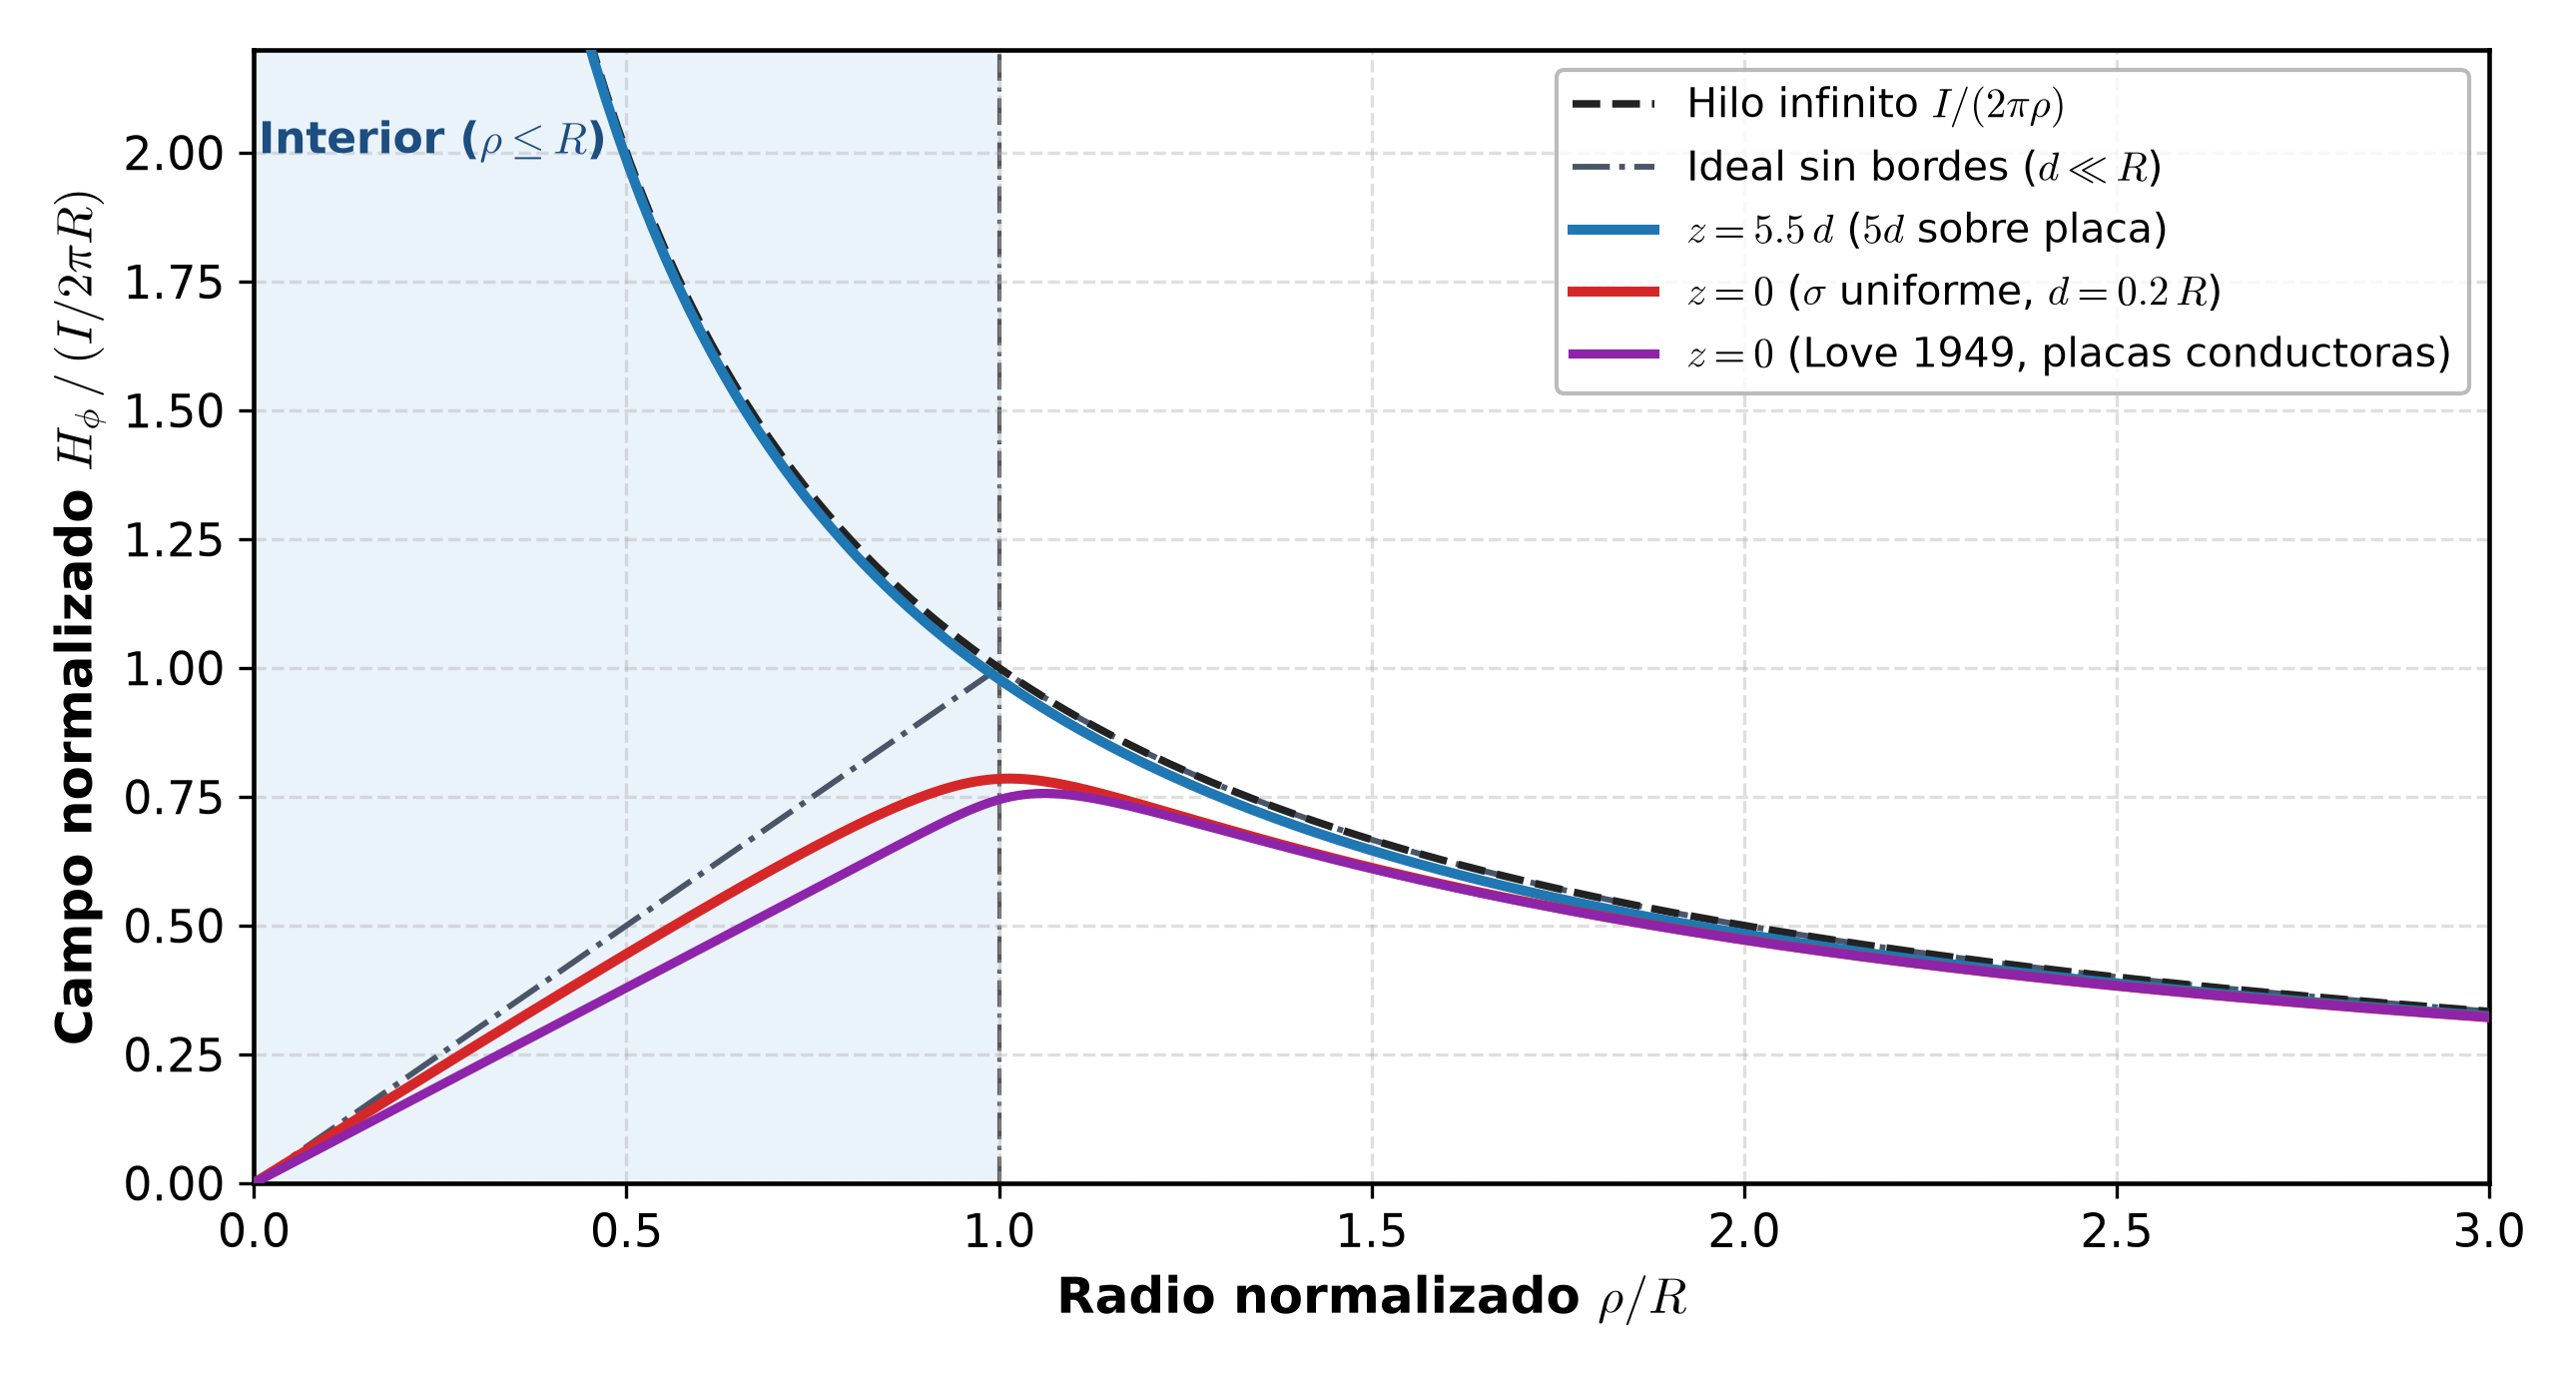
\includegraphics[width=0.95\textwidth]{perfil_radial_baja_frecuencia_v2.png}%
}{%
    \framebox{\parbox{0.85\textwidth}{\centering\vspace{1cm}\texttt{perfil\_radial\_baja\_frecuencia\_v2.png}\\[0.2cm]{\small\color{mutedgray}(Imagen externa no disponible en la vista previa; se insertará automáticamente cuando el archivo PNG esté en la misma carpeta)}\vspace{1cm}}}%
}
\caption{Perfil radial del campo magnético normalizado $H_\phi / (I / 2\pi R)$ para $d = 0{,}2\,R$, generado por \texttt{perfil\_radial\_baja\_frecuencia\_v2.py}. Se comparan el hilo infinito, el límite ideal sin bordes, el plano $z = 5{,}5\,d$ y el plano medio $z = 0$ tanto con densidad de carga uniforme como con la solución exacta de Love (1949).}
\label{fig:perfil-radial}
\end{figure}

\end{document}